\documentclass[15pt,a5paper,reqno]{article}
\usepackage{hyperref}
\usepackage[warn]{mathtext}
\usepackage[utf8]{inputenc}
\usepackage[T2A]{fontenc}
\usepackage[russian]{babel}
\usepackage{amssymb, amsmath, multicol}
\usepackage{graphicx}
\usepackage[shortcuts,cyremdash]{extdash}
\usepackage{wrapfig}
\usepackage{floatflt}
\usepackage{lipsum}
\usepackage{verbatim}
\usepackage{concmath}
\usepackage{euler}
\usepackage{xcolor}
\usepackage{etoolbox}
\usepackage{fancyhdr}
\usepackage{subfiles}
\usepackage{enumitem}
\usepackage{amsthm}
\usepackage{indentfirst}
\usepackage{import}

\DeclareMathOperator{\sign}{sign}

\RequirePackage[ left     = 1.5cm,
  right    = 1.5cm,
  top      = 2.0cm,
  bottom   = 1.25cm,
  includefoot,
  footskip = 1.25cm ]{geometry}
\setlength    {\parskip}        { .5em plus .15em minus .08em }
%\setlength    {\parindent}      { .0em }
\renewcommand {\baselinestretch}{ 1.07 }

\fancyhf{}

\renewcommand{\footrulewidth}{ .0em }
\fancyfoot[C]{\texttt{\textemdash~\thepage~\textemdash}}
\fancyhead[R]{\hfilШурыгин}

\makeatletter
\patchcmd\l@section{%
  \nobreak\hfil\nobreak
}{%
  \nobreak
  \leaders\hbox{%
    $\m@th \mkern \@dotsep mu\hbox{.}\mkern \@dotsep mu$%
  }%
  \hfill
  \nobreak
}{}{\errmessage{\noexpand\l@section could not be patched}}
\makeatother
\parindent = 1cm % отступ при красной строке⏎
\pagestyle{fancy}    
\renewcommand\qedsymbol{$\blacksquare$}

\newcommand{\when}[2]{
  \left. #1 \right|_{#2} \hspace
}
\renewcommand{\kappa}{\varkappa}
\RequirePackage{caption2}
\renewcommand\captionlabeldelim{}
\newcommand*{\hm}[1]{#1\nobreak\discretionary{}

\DeclareSymbolFont{T2Aletters}{T2A}{cmr}{m}{it}
{\hbox{$\mathsurround=0pt #1$}}{}}
% Цвета для гиперссылок
\definecolor{linkcolor}{HTML}{000000} % цвет ссылок
\definecolor{urlcolor}{HTML}{799B03} % цвет гиперссылок
 
\hypersetup{pdfstartview=FitH,  linkcolor=linkcolor,urlcolor=urlcolor, colorlinks=true}


%\setcounter{secnum[utf8x]depth}{0}

\begin{document}

% НАЧАЛО ТИТУЛЬНОГО ЛИСТА
\begin{center}
  {\small ФЕДЕРАЛЬНОЕ ГОСУДАРСТВЕННОЕ АВТОНОМНОЕ ОБРАЗОВАТЕЛЬНОЕ\\ УЧРЕЖДЕНИЕ ВЫСШЕГО ОБРАЗОВАНИЯ\\ МОСКОВСКИЙ ФИЗИКО-ТЕХНИЧЕСКИЙ ИНСТИТУТ\\ (НАЦИОНАЛЬНЫЙ ИССЛЕДОВАТЕЛЬСКИЙ УНИВЕРСИТЕТ)\\ ФИЗТЕХ-ШКОЛА РАДИОТЕХНИКИ И КИБЕРНЕТИКИ}\\
  \hfill \break
  \hfill \break
  \hfill \break
  \Huge{Исследование энергетич. спектра $\beta$ -- частиц, определение их макс. энерг. магнитным спектрометром}\\
\end{center}

\hfill \break
\hfill \break
\hfill \break
\hfill \break
\hfill \break
\hfill \break

\begin{flushright}
  \normalsize{Работу выполнил:}\\
  \normalsize{\textbf{Шурыгин Антон Алексеевич, группа Б01-909}}\\
\end{flushright}

\begin{center}
  \normalsize{\textbf{Долгопрудный, 2021}}
\end{center}


\thispagestyle{empty} % выключаем отображение номера для этой страницы

% КОНЕЦ ТИТУЛЬНОГО ЛИСТА

\newpage
\thispagestyle{plain}
\tableofcontents
\thispagestyle{plain}
\newpage


\paragraph{Цель работы:}
Исследование энергетического спектра $\beta$-частиц при распаде ядер $^{137}$Cs и определение их максимальной энергии при помощи магнитного спектрометра. 

\paragraph
{В работе используются:}
\begin{itemize}
    \item Магнитный спектрометр с <<короткой линзой>>
    \item Высоковольтный и низковольтный выпрямители
    \item Форвакуумный насос и вакуумметр
    \item ЭВМ
\end{itemize}

\section{Теоретические положения}

\textbf{Бета-распад} --  это самопроизвольное превращение ядер, при котором их массовое число не изменяется, а заряд изменяется на единицу. В данной работе мы будем иметь дело с электронным распадом:
		\begin{equation}
		    _{Z}^{A}X \rightarrow _{Z+1}^{A}X + e^{-} + \widetilde{\nu}
		\end{equation}
		Освобождающаяся в результате распада энергия делится между исходным ядром, электроном и нейтрино. При этом доля энергии, уносимая ядром крайне мала, так что вся энергия делится между нейтрино и электроном. Поэтому электроны могут иметь любую энергию от нулевой до некоторой максимальной энергии, высвобождаемой при распаде.
		
		Вероятность $\omega$ того, что электрон вылетит с импульсом $^3p$, а нейтрино с импульсом $^3k$ равна произведению этих дифференциалов, но мы должны учесть также закон сохранения энергии.
		\begin{equation}
		    E_e - E - ck = 0
		\end{equation}
		Энергия электрона связана с импульсом обычным образом:
		\begin{equation}
		    E = c\sqrt{p^2 + m^2c^2} -mc^2
		\end{equation}
		Таким образом, вероятность $\omega$ принимает вид:
		\begin{equation}
		    \omega = D\delta(E_e-E-ck)^3p^3k = D\delta(E_e-E-ck)p^2 pk^2 k\Omega_e\Omega_{\widetilde{\nu}}
		\end{equation}
		D можно считать с хорошей точностью константой. В этом случае можно проинтегрировать по всем углам и по абсолютному значению импульса нейтрино. В этом случае $\delta$-функция исчезнет, а $ck$ всюду заменится на $E_e-E$. После умножения на полное число распадов выражение примет вид:
		\begin{equation}
		     N = \frac{16\pi^2N_0}{c^2} D p^2\left(E_e-E\right)^2 p
		\end{equation}
		В нерелятивистском случае выражение упрощается и принимает вид:
		\begin{equation}
			\frac{ N}{ E} \simeq \sqrt{E}(E_e - E)^2
		\end{equation}
		
		Дочерние ядра, возникающие в результате $\beta$-распада, нередко оказываются возбуждёнными. Возбуждённые ядра отдают свою энергию либо излучая гамма-квант, либо передавая избыток энергии одному из электронов с внутренних оболочек атома (обычно $K$ или $L$). Последние электроны имеют строго определённую энергию и называются \textit{конверсионными}. Ширина монохроматической линии, соответствующая конверсионным электронам, определяет разрешающую силу спектрометра.

\section{Экспериментальная установка}

    \begin{figure}[h]
\begin{center}
\begin{minipage}[h]{0.48\linewidth}
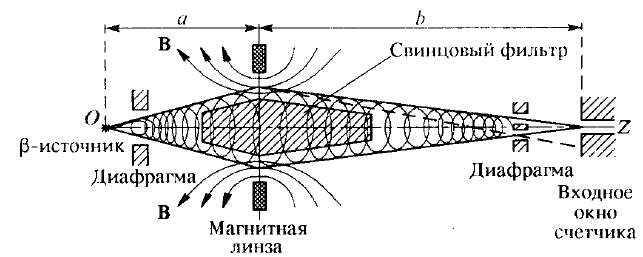
\includegraphics[width=1\linewidth]{pics/lens_5_4_2.png}
\caption{Схема $\beta$-спектрометра с короткой магнитной линзой} %% подпись к рисунку\label{ris:experimoriginal} %% метка рисунка для ссылки на него
\end{minipage}
\hfill 
\begin{minipage}[h]{0.48\linewidth}
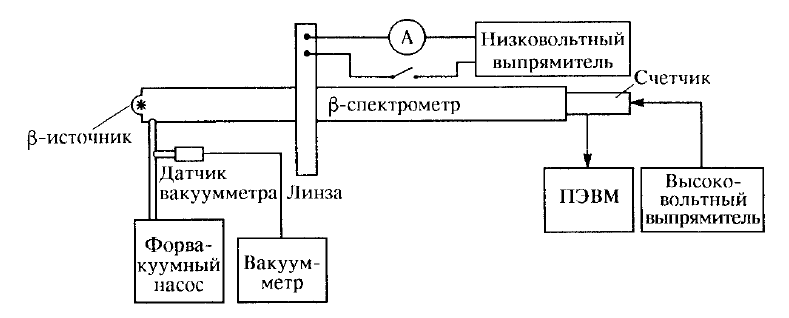
\includegraphics[width=1\linewidth]{pics/stff_5_4_2.png}
\caption{Блок-схема установки для изучения $\beta$-спектра}
\label{ris:experimcoded}
\end{minipage}
\end{center}
\end{figure}

Энергию частиц определяют с помощью $\beta$-спектрометров. В работе используется магнитный спектрометр с <<короткой>> линзой, сцинтиллятором и ФЭУ. Как показывает расчет, для заряженных частиц тонкая катушка эквивалентна линзе:
		\begin{equation}
			\frac{1}{f} \simeq \frac{I^2}{p_e^2}
		\end{equation}
	При заданной силе тока на входное окно счетчика собираются электроны с определенным импульсом. Импульс сфокусированных электронов пропорционален силе тока, коэффициент пропорциональности определяется по какой-либо известной конверсионной линии. \par
	Давление в спектрометре поддерживается на уровне около 0,1 Торр и измеряется термопарным вакуумметром. Откачка осуществляется форвакуумным насосом. Высокое напряжение на ФЭУ подаётся от стабилизированного выпрямителя.

\section{Выполнение работы и обработка данных}

\begin{enumerate}
    \item Откачаем воздух из полости спектрометра. включим формирователь импульсов и питание магнитной линзы.
    \item Изменяя ток линзы через 0,2 А, проведём измерение зависимости интенсивности потока падающих $\beta$-частиц от силы тока, время накопления - 100 секунд. Более подробно пропишем конверсионный спектр. Результаты измерения занесём в таблицу 1.
    \item Проведём измерение фона - фонового излучения нет.
    \item Прокалибруем спектрометр с учётом того, что $p_{conv}c = $1013.5 кэВ ($p_{conv} = 634 $кэВ у $^{137}$Cs). Определим значения энергии, импульса и величину $\frac{\sqrt{N(p)}}{p^{3/2}}$ для построения графика Ферми-Кюри.
    \item Построим графики зависимости интенсивности потока частиц от силы тока (рис. 3) и график Ферми-Кюри (рис. 4)
    
    \item По графику Ферми-Кюри определим максимальную энергию 

		  $\beta$-частиц в спектре, $E_{max} = $ 567,22 кэВ

  
\subsection{Анализ погрешностей}

\begin{table}[h!]
	\centering
	\begin{tabular}{| c | c | c | c |}
\hline
$I, A$ & $N - N_ф, 1/c$ & $\sigma_{N - N_ф}, 1/c$ & $\sigma_{I}$\\
    \hline
    $0,1$ & $-0,204$ & $0$ & $0,001$\\
    \hline
    $0,2$ & $-0,353$ & $0$ & $0,001$\\
    \hline
    $0,3$ & $-0,184$ & $0$ & $0,001$\\
    \hline
    $0,4$ & $0,186$ & $0,019$ & $0,001$\\
    \hline
    $0,5$ & $0,176$ & $0,018$ & $0,001$\\
    \hline
    $0,6$ & $0,066$ & $0,007$ & $0,001$\\
    \hline
    $0,7$ & $0,416$ & $0,042$ & $0,001$\\
    \hline
    $0,8$ & $0,816$ & $0,082$ & $0,001$\\
    \hline
    $0,9$ & $1,216$ & $0,122$ & $0,001$\\
    \hline
    $0,95$ & $2,026$ & $0,203$ & $0,001$\\
    \hline
    $1$ & $2,905$ & $0,291$ & $0,001$\\
    \hline
    $1,1$ & $3,515$ & $0,352$ & $0,001$\\
    \hline
    $1,15$ & $3,975$ & $0,398$ & $0,001$\\
    \hline
    $1,2$ & $4,725$ & $0,473$ & $0,001$\\
    \hline
    $1,3$ & $5,955$ & $0,596$ & $0,001$\\
    \hline
    $1,4$ & $6,254$ & $0,625$ & $0,001$\\
    \hline
    $1,5$ & $7,304$ & $0,73$ & $0,001$\\
    \hline
    $1,6$ & $7,614$ & $0,761$ & $0,001$\\
    \hline
    $1,7$ & $8,134$ & $0,813$ & $0,001$\\
    \hline
    $1,8$ & $8,204$ & $0,82$ & $0,001$\\
\hline
\end{tabular}

	\caption{: данные для графика спектра}
	\label{tb1}
\end{table}


\begin{table}[h!]
	\centering
	\begin{tabular}{| c | c | c | c |}
    \hline
    $I, A$ & $N - N_ф, 1/c$ & $\sigma_{N - N_ф}, 1/c$ & $\sigma_{I}$\\
    \hline
    $1,9$ & $7,024$ & $0,702$ & $0,001$\\
    \hline
    $2$ & $7,074$ & $0,707$ & $0,001$\\
    \hline
    $2,1$ & $6,904$ & $0,69$ & $0,001$\\
    \hline
    $2,2$ & $6,154$ & $0,615$ & $0,001$\\
    \hline
    $2,3$ & $5,195$ & $0,52$ & $0,001$\\
    \hline
    $2,4$ & $4,425$ & $0,443$ & $0,001$\\
    \hline
    $2,5$ & $3,865$ & $0,387$ & $0,001$\\
    \hline
    $2,6$ & $2,506$ & $0,251$ & $0,001$\\
    \hline
    $2,7$ & $2,176$ & $0,218$ & $0,001$\\
    \hline
    $2,8$ & $1,516$ & $0,152$ & $0,001$\\
    \hline
    $2,9$ & $1,686$ & $0,169$ & $0,001$\\
    \hline
    $3$ & $2,685$ & $0,269$ & $0,001$\\
    \hline
    $3,1$ & $3,895$ & $0,39$ & $0,001$\\
    \hline
    $3,15$ & $4,595$ & $0,46$ & $0,001$\\
    \hline
    $3,2$ & $3,675$ & $0,368$ & $0,001$\\
    \hline
    $3,25$ & $2,166$ & $0,217$ & $0,001$\\
    \hline
    $3,3$ & $0,976$ & $0,098$ & $0,001$\\
    \hline
    $3,4$ & $-0,124$ & $-0,012$ & $0,001$\\
    \hline
    $3,5$ & $-0,654$ & $-0,065$ & $0,001$\\
    \hline
    $3,6$ & $-0,694$ & $-0,069$ & $0,001$\\
    \hline
    $3,7$ & $0,426$ & $0,043$ & $0,001$\\
    \hline
    $3,8$ & $0,486$ & $0,049$ & $0,001$\\
    \hline
    $3,9$ & $0,776$ & $0,078$ & $0,001$\\
    \hline
    $4$ & $0,326$ & $0,033$ & $0,001$\\
    \hline
    \end{tabular}
	\caption{: данные для графика спектра}
	\label{tb2}
\end{table}

\begin{table}[h!]
	\centering
	\begin{tabular}{| c | c | c |}
\hline
$T, кэВ$ & $mkFermi$ & $\sigma_{mkFermi}$\\
    \hline
    $1$ & $0$ & $0$\\
    \hline
    $4$ & $0$ & $0$\\
    \hline
    $9,1$ & $0$ & $0$\\
    \hline
    $16$ & $295,02$ & $14,77$\\
    \hline
    $24,8$ & $205,35$ & $10,28$\\
    \hline
    $35,3$ & $95,76$ & $4,79$\\
    \hline
    $47,5$ & $190,51$ & $9,53$\\
    \hline
    $61,3$ & $218,36$ & $10,92$\\
    \hline
    $76,5$ & $223,38$ & $11,17$\\
    \hline
    $84,6$ & $265,87$ & $13,3$\\
    \hline
    $93,1$ & $294,83$ & $14,74$\\
    \hline
    $110,8$ & $281,1$ & $14,06$\\
    \hline
    $120,1$ & $279,64$ & $13,98$\\
    \hline
    $129,7$ & $286,02$ & $14,3$\\
    \hline
    $149,7$ & $76$ & $3,8$\\
    \hline
    $170,5$ & $261,14$ & $13,06$\\
    \hline
    $192,3$ & $245,6$ & $12,28$\\
    \hline
    $214,8$ & $235,83$ & $11,79$\\
    \hline
    $238,8$ & $222,56$ & $11,13$\\
    \hline
    $261,8$ & $205,15$ & $10,26$\\
    \hline
\end{tabular}

	\caption{: данные для графика}
	\label{tb3}
\end{table}


\begin{table}[h!]
	\centering
	\begin{tabular}{| c | c | c |}
    \hline
    $T, кэВ$ & $mkFermi$ & $\sigma_{mkFermi}$\\
    \hline
    $286,3$ & $175,04$ & $8,75$\\
    \hline
    $311,3$ & $162,65$ & $8,13$\\
    \hline
    $336,8$ & $149,35$ & $7,47$\\
    \hline
    $362,7$ & $131,5$ & $6,58$\\
    \hline
    $389$ & $113,5$ & $5,68$\\
    \hline
    $415,7$ & $97,86$ & $4,89$\\
    \hline
    $442,7$ & $86,03$ & $4,3$\\
    \hline
    $470,1$ & $65,3$ & $3,27$\\
    \hline
    $497,7$ & $57,5$ & $2,88$\\
    \hline
    $525,6$ & $45,45$ & $2,27$\\
    \hline
    $553,8$ & $45,47$ & $2,27$\\
    \hline
    $582,1$ & $54,55$ & $2,73$\\
    \hline
    $610,7$ & $62,54$ & $3,13$\\
    \hline
    $625,1$ & $66,32$ & $3,32$\\
    \hline
    $639,5$ & $57,92$ & $2,9$\\
    \hline
    $653,9$ & $43,44$ & $2,17$\\
    \hline
    $668,4$ & $28,5$ & $1,43$\\
    \hline
    $697,5$ & $0$ & $0$\\
    \hline
    $726,8$ & $0$ & $0$\\
    \hline
    $756,2$ & $0$ & $0$\\
    \hline
    $785,8$ & $15,86$ & $0,79$\\
    \hline
    $815,4$ & $16,28$ & $0,81$\\
    \hline
    $845,2$ & $19,78$ & $0,99$\\
    \hline
    $875,1$ & $12,34$ & $0,62$\\
    \hline
    \end{tabular}
	\caption{.2: данные для графика}
	\label{tb4}
\end{table}


При измерениях радиационного фона $N_ф$ за погрешность бралось $10 \%$ от полученной величины.

В последствии такую же долю погрешности я брал при использовании данных из столбца $N - N_ф$. Результаты вычисления погрешности занесены в таблицу \ref{tb1}, \ref{tb2}, столбец $\sigma_{N - N_ф}$.

\textbf{Оценка остальных погрешностей}

\begin{itemize}
	\item $\sigma_{I} \approx$ 0.001 A
	\item $\sigma_{mkFermi} = mkFermi \cdot \sqrt{\frac{1}{2}\left(\frac{\sigma_{N - N_ф}^{2}}{N - N_ф} \right) + \frac{3}{2}\left(\frac{\sigma_{I}}{I}\right)^{2}} $
\end{itemize}

\begin{figure}[h!]
			\centering
			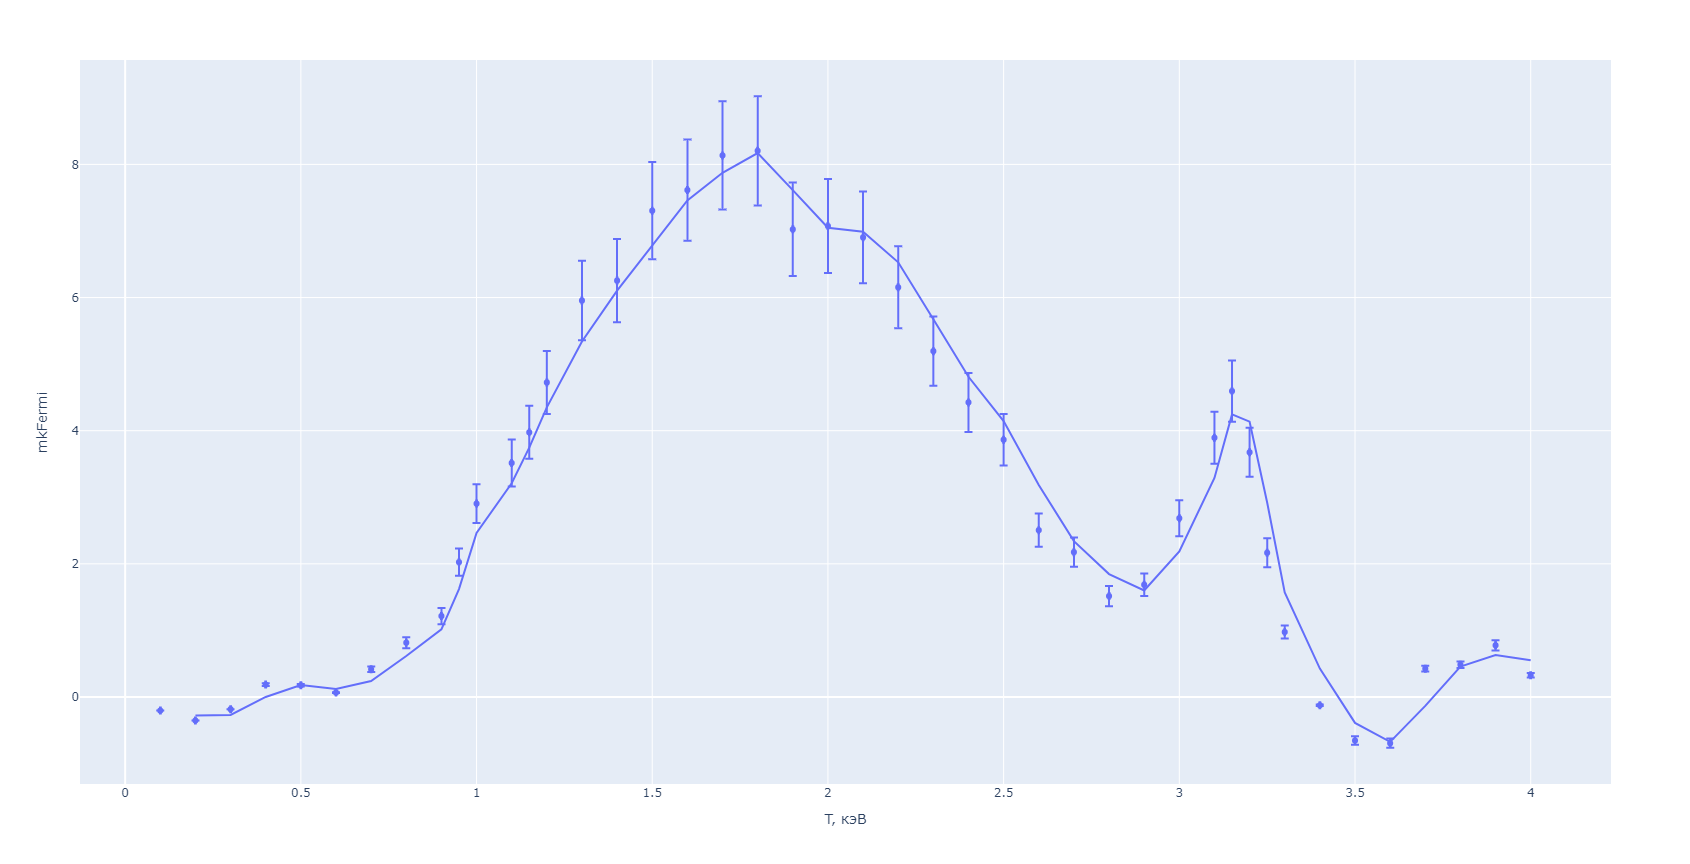
\includegraphics[width=\linewidth]{pics/lab_5_4_2_1.png}
			\caption{Зависимость интенсивности потока частиц от силы тока в магнитной линзе}
		\end{figure}
		
\begin{figure}[h!]
			\centering
			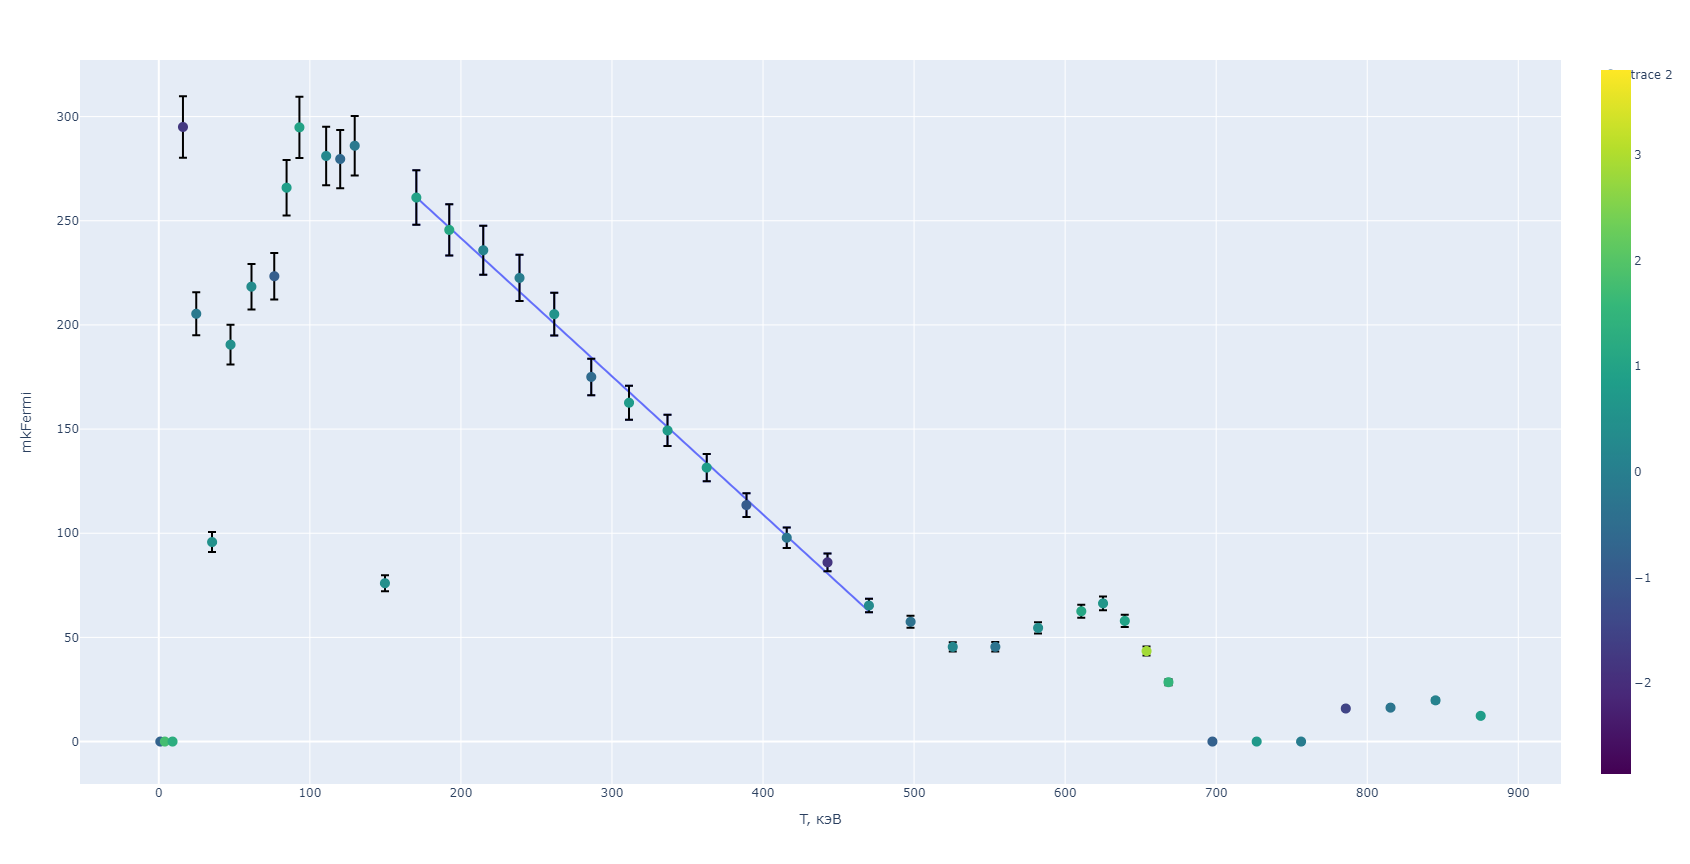
\includegraphics[width=\linewidth]{pics/lab_5_4_2_2.png}
			\caption{График Ферми-Кюри}
		\end{figure}
		
\end{enumerate}


\section{Вывод}
	В ходе работы было исследовано явление $\beta$-распада $^{137}$Cs. В спектре $\beta$-частиц наблюдаются две области: электроны, рождённые в паре с антинейтрино (приближаемая по Лоренцу кривая на графике спектра) и конверсионные электроны, испускаемые в результате перехода ядра на более низкий энергетический уровень (монохроматическая линия, строго определённое значение энергии 634 кэВ). \par
	Также с помощью графика Ферми-Кюри ($\frac{\sqrt{N}}{p^{3/2}} = f(T_{kin})$) было определено максимальное значение энергии $\beta$-частиц в спектре: $E_{max} = $ 567,22 кэВ
	Полученное значение отличается приблизительно на $10 \%$ от $E_{conv} = 634$ кэВ, т.е. результат находится в пределах погрешности взятой для измерения числа электронов.

\end{document}